\documentclass{standalone}
\usepackage{tikz}
\usetikzlibrary{patterns, positioning}


\begin{document}
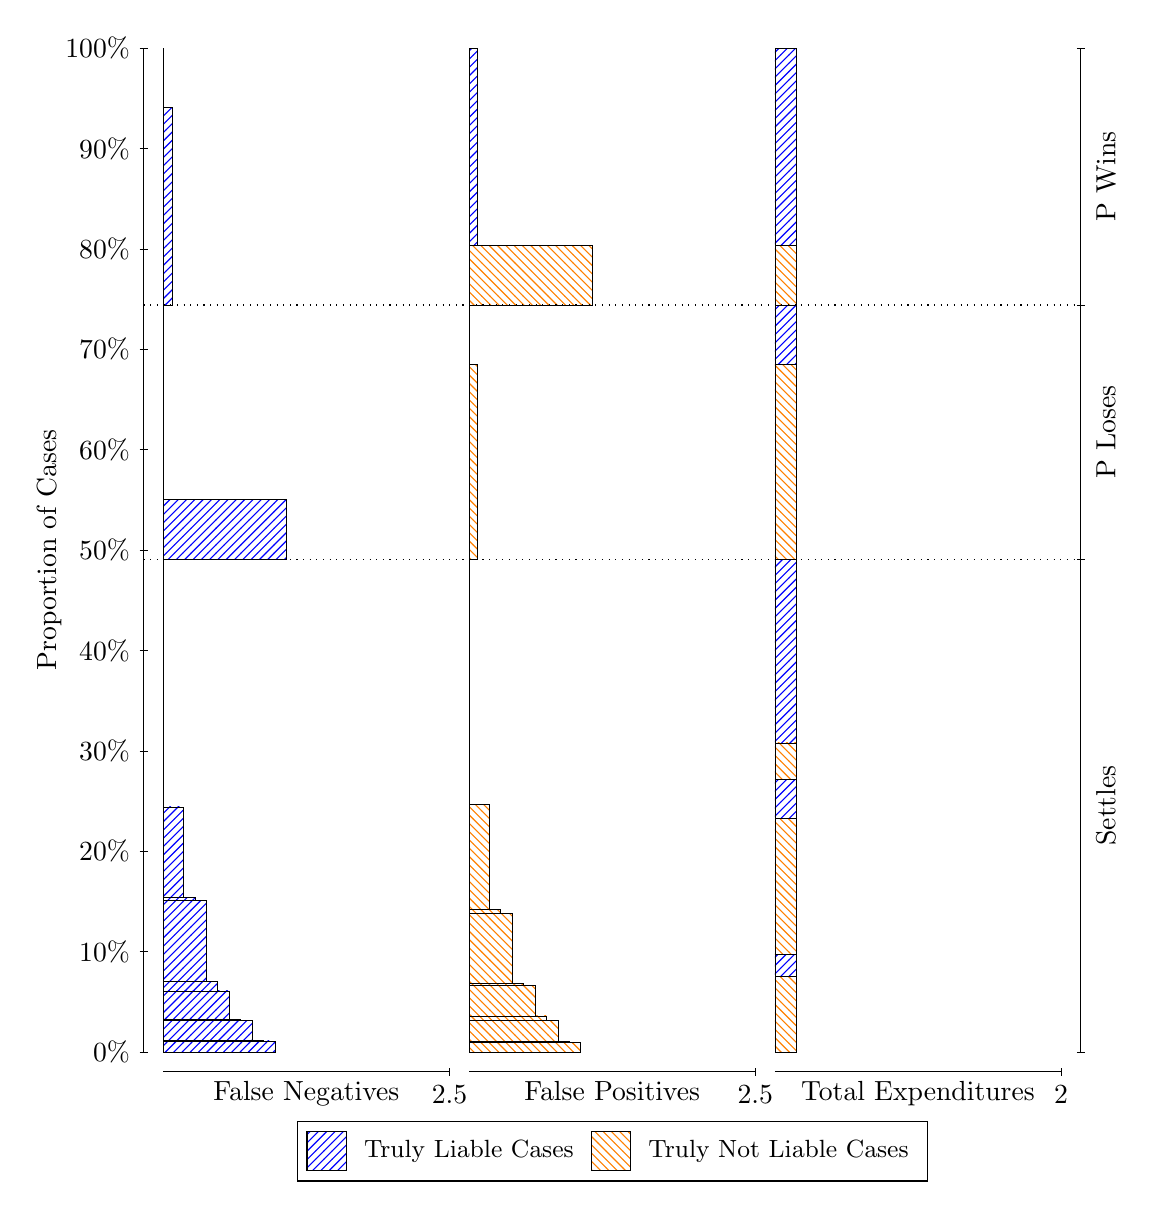
\begin{tikzpicture}
\draw[black, very thin] (1.5,1.75) -- (1.5,14.5);
\node[rotate=90, text=black, anchor=center] at (0.3, 8.125) {Proportion of Cases};
\draw[black, very thin] (1.45,1.75) -- (1.55,1.75);
\node[text=black, anchor=east] at (1.45, 1.75) {0\%};
\draw[black, very thin] (1.45,3.025) -- (1.55,3.025);
\node[text=black, anchor=east] at (1.45, 3.025) {10\%};
\draw[black, very thin] (1.45,4.3) -- (1.55,4.3);
\node[text=black, anchor=east] at (1.45, 4.3) {20\%};
\draw[black, very thin] (1.45,5.575) -- (1.55,5.575);
\node[text=black, anchor=east] at (1.45, 5.575) {30\%};
\draw[black, very thin] (1.45,6.85) -- (1.55,6.85);
\node[text=black, anchor=east] at (1.45, 6.85) {40\%};
\draw[black, very thin] (1.45,8.125) -- (1.55,8.125);
\node[text=black, anchor=east] at (1.45, 8.125) {50\%};
\draw[black, very thin] (1.45,9.4) -- (1.55,9.4);
\node[text=black, anchor=east] at (1.45, 9.4) {60\%};
\draw[black, very thin] (1.45,10.675) -- (1.55,10.675);
\node[text=black, anchor=east] at (1.45, 10.675) {70\%};
\draw[black, very thin] (1.45,11.95) -- (1.55,11.95);
\node[text=black, anchor=east] at (1.45, 11.95) {80\%};
\draw[black, very thin] (1.45,13.225) -- (1.55,13.225);
\node[text=black, anchor=east] at (1.45, 13.225) {90\%};
\draw[black, very thin] (1.45,14.5) -- (1.55,14.5);
\node[text=black, anchor=east] at (1.45, 14.5) {100\%};

\draw[black, very thin] (13.4,1.75) -- (13.4,14.5);
\draw[black, very thin] (13.35,1.75) -- (13.45,1.75);
\node[anchor=west] at (13.35, 1.75) {};
\draw[black, very thin] (13.35,8.0095) -- (13.45,8.0095);
\node[anchor=west] at (13.35, 8.0095) {};
\draw[black, very thin] (13.35,11.236) -- (13.45,11.236);
\node[anchor=west] at (13.35, 11.236) {};
\draw[black, very thin] (13.35,14.5) -- (13.45,14.5);
\node[anchor=west] at (13.35, 14.5) {};

\draw[black, very thin, pattern color=blue, pattern=north east lines] (1.75,1.75) rectangle (3.167,1.8915);
\draw[black, very thin, pattern color=blue, pattern=north east lines] (1.75,1.8915) rectangle (3.0217,1.9);
\draw[black, very thin, pattern color=blue, pattern=north east lines] (1.75,1.9) rectangle (2.8763,2.1527);
\draw[black, very thin, pattern color=blue, pattern=north east lines] (1.75,2.1527) rectangle (2.731,2.1646);
\draw[black, very thin, pattern color=blue, pattern=north east lines] (1.75,2.1646) rectangle (2.5857,2.5259);
\draw[black, very thin, pattern color=blue, pattern=north east lines] (1.75,2.5259) rectangle (2.4403,2.6418);
\draw[black, very thin, pattern color=blue, pattern=north east lines] (1.75,2.6418) rectangle (2.295,3.671);
\draw[black, very thin, pattern color=blue, pattern=north east lines] (1.75,3.671) rectangle (2.1497,3.7147);
\draw[black, very thin, pattern color=blue, pattern=north east lines] (1.75,3.7147) rectangle (2.0043,4.8612);
\draw[black, very thin, pattern color=orange, pattern=north west lines] (1.75,4.8612) rectangle (1.75,8.0095);
\draw[black, very thin, pattern color=blue, pattern=north east lines] (1.75,8.0095) rectangle (3.3123,8.7653);
\draw[black, very thin, pattern color=orange, pattern=north west lines] (1.75,8.7653) rectangle (1.75,11.236);
\draw[black, very thin, pattern color=blue, pattern=north east lines] (1.75,11.236) rectangle (1.859,13.744);
\draw[black, very thin, pattern color=orange, pattern=north west lines] (1.75,13.744) rectangle (1.75,14.5);
\draw[black, very thin, pattern color=orange, pattern=north west lines] (5.6333,1.75) rectangle (7.0503,1.8749);
\draw[black, very thin, pattern color=orange, pattern=north west lines] (5.6333,1.8749) rectangle (6.905,1.8834);
\draw[black, very thin, pattern color=orange, pattern=north west lines] (5.6333,1.8834) rectangle (6.7597,2.1557);
\draw[black, very thin, pattern color=orange, pattern=north west lines] (5.6333,2.1557) rectangle (6.6143,2.2093);
\draw[black, very thin, pattern color=orange, pattern=north west lines] (5.6333,2.2093) rectangle (6.469,2.5953);
\draw[black, very thin, pattern color=orange, pattern=north west lines] (5.6333,2.5953) rectangle (6.3237,2.6189);
\draw[black, very thin, pattern color=orange, pattern=north west lines] (5.6333,2.6189) rectangle (6.1783,3.5132);
\draw[black, very thin, pattern color=orange, pattern=north west lines] (5.6333,3.5132) rectangle (6.033,3.5568);
\draw[black, very thin, pattern color=orange, pattern=north west lines] (5.6333,3.5568) rectangle (5.8877,4.8984);
\draw[black, very thin, pattern color=blue, pattern=north east lines] (5.6333,4.8984) rectangle (5.6333,8.0095);
\draw[black, very thin, pattern color=orange, pattern=north west lines] (5.6333,8.0095) rectangle (5.7423,10.48);
\draw[black, very thin, pattern color=blue, pattern=north east lines] (5.6333,10.48) rectangle (5.6333,11.236);
\draw[black, very thin, pattern color=orange, pattern=north west lines] (5.6333,11.236) rectangle (7.1957,11.992);
\draw[black, very thin, pattern color=blue, pattern=north east lines] (5.6333,11.992) rectangle (5.7423,14.5);
\draw[black, very thin, pattern color=orange, pattern=north west lines] (9.5167,1.75) rectangle (9.7892,2.7115);
\draw[black, very thin, pattern color=blue, pattern=north east lines] (9.5167,2.7115) rectangle (9.7892,2.9846);
\draw[black, very thin, pattern color=orange, pattern=north west lines] (9.5167,2.9846) rectangle (9.7892,4.7121);
\draw[black, very thin, pattern color=blue, pattern=north east lines] (9.5167,4.7121) rectangle (9.7892,5.215);
\draw[black, very thin, pattern color=orange, pattern=north west lines] (9.5167,5.215) rectangle (9.7892,5.6743);
\draw[black, very thin, pattern color=blue, pattern=north east lines] (9.5167,5.6743) rectangle (9.7892,8.0095);
\draw[black, very thin, pattern color=orange, pattern=north west lines] (9.5167,8.0095) rectangle (9.7892,10.48);
\draw[black, very thin, pattern color=blue, pattern=north east lines] (9.5167,10.48) rectangle (9.7892,11.236);
\draw[black, very thin, pattern color=orange, pattern=north west lines] (9.5167,11.236) rectangle (9.7892,11.992);
\draw[black, very thin, pattern color=blue, pattern=north east lines] (9.5167,11.992) rectangle (9.7892,14.5);
\draw[black, dotted] (1.5,8.0095) -- (13.4,8.0095);
\draw[black, dotted] (1.5,11.236) -- (13.4,11.236);
\draw[black, very thin] (1.75,1.5) -- (5.3833,1.5);
\node[text=black, anchor=north] at (3.5667, 1.5) {False Negatives};
\draw[black, very thin] (5.3833,1.45) -- (5.3833,1.55);
\node[text=black, anchor=north] at (5.3833, 1.45) {2.5};

\draw[black, very thin] (5.6333,1.5) -- (9.2667,1.5);
\node[text=black, anchor=north] at (7.45, 1.5) {False Positives};
\draw[black, very thin] (9.2667,1.45) -- (9.2667,1.55);
\node[text=black, anchor=north] at (9.2667, 1.45) {2.5};

\draw[black, very thin] (9.5167,1.5) -- (13.15,1.5);
\node[text=black, anchor=north] at (11.333, 1.5) {Total Expenditures};
\draw[black, very thin] (13.15,1.45) -- (13.15,1.55);
\node[text=black, anchor=north] at (13.15, 1.45) {2};

\node[text=black, centered, rotate=90] at (13.72, 4.8798) {Settles};
\node[text=black, centered, rotate=90] at (13.72, 9.6227) {P Loses};
\node[text=black, centered, rotate=90] at (13.72, 12.868) {P Wins};

\draw (7.449999999999999,1.5) node[draw=none] (baseCoordinate) {};
\begin{scope}[align=center]
        \matrix[scale=0.5, draw=black, below=0.5cm of baseCoordinate, nodes={draw}, column sep=0.1cm]{
            \node[rectangle, draw, minimum width=0.5cm, minimum height=0.5cm, pattern color=blue, pattern=north east lines] {}; &
            \node[draw=none, font=\small, text=black] (B) {Truly Liable Cases}; &
            \node[rectangle, draw, minimum width=0.5cm, minimum height=0.5cm, pattern color=orange, pattern=north west lines] {}; &
            \node[draw=none, font=\small, text=black] (B) {Truly Not Liable Cases}; \\
            };
\end{scope}

\end{tikzpicture}
\end{document}